%% jsc_paper_main.tex
%% Waring decomposition of derivatives and its applications
%%
%% Target journal: Journal of Computational Physics
%% Document class: siamltex (SIAM)
%% Build sequence: pdflatex, bibtex, pdflatex, pdflatex.

\documentclass[final,oneeqnum]{siamltex}

%% ========== Packages ==========
\usepackage{amsmath,amssymb}
\usepackage{mathrsfs}
%% Note: amsthm is NOT loaded because siamltex.cls defines its own proof environment
\usepackage{mathtools}
\usepackage{bm}
\usepackage{graphicx}
\usepackage{booktabs}
\usepackage{algorithm}
\usepackage{cite}
\usepackage{hyperref}
\usepackage{cleveref}
\usepackage{aliascnt}
\usepackage{enumitem}
\usepackage{xcolor}
\usepackage{multirow}
\usepackage{placeins}

%% Keep appendix floats ahead of the bibliography without changing its source.
\let\originalbibliography\bibliography
\renewcommand{\bibliography}[1]{\FloatBarrier\originalbibliography{#1}}

\hypersetup{hidelinks}
\graphicspath{{figures/}}

%% Hyperref anchors must include the section because siamltex resets floats.
\renewcommand{\theHtable}{\thesection.\arabic{table}}
\renewcommand{\theHfigure}{\thesection.\arabic{figure}}

%% ========== Float placement ==========
\makeatletter
\setlength{\@fptop}{0pt}
\setlength{\@fpbot}{0pt plus 1fil}
\makeatother
\renewcommand{\topfraction}{0.88}
\renewcommand{\bottomfraction}{0.85}
\renewcommand{\textfraction}{0.10}
\renewcommand{\floatpagefraction}{0.70}

%% ========== Math Operators ==========
%% Note: \rank and \diag are already provided by siamltex.cls

%% ========== Theorem Environments ==========
%% theorem, lemma, corollary, proposition, definition are defined by siamltex.cls
%% Number definitions separately; propositions retain the shared theorem counter.
\let\definition\relax
\let\enddefinition\relax
\newtheorem{definition}{Definition}[section]
\crefname{definition}{Definition}{Definitions}
\Crefname{definition}{Definition}{Definitions}

%% Use aliascnt so that cleveref identifies remark/example types while sharing
%% the theorem counter for unified numbering.
\newaliascnt{remark}{theorem}
\newtheorem{remark}[remark]{Remark}
\aliascntresetthe{remark}
\crefname{remark}{Remark}{Remarks}
\Crefname{remark}{Remark}{Remarks}

\newaliascnt{example}{theorem}
\newtheorem{example}[example]{Example}
\aliascntresetthe{example}
\crefname{example}{Example}{Examples}
\Crefname{example}{Example}{Examples}

%% ========== Custom Commands ==========
\newcommand{\R}{\mathbb{R}}
\newcommand{\C}{\mathbb{C}}
\newcommand{\N}{\mathbb{N}}
\newcommand{\Z}{\mathbb{Z}}
\newcommand{\E}{\mathbb{E}}
\newcommand{\bx}{\bm{x}}
\newcommand{\bz}{\bm{z}}
\newcommand{\bv}{\bm{v}}
\newcommand{\Tp}{T_{p}}
\newcommand{\norm}[1]{\left\|#1\right\|}
\newcommand{\abs}[1]{\left|#1\right|}

\emergencystretch=1.5em

\begin{document}

%% ========== Title ==========
\title{Waring Decomposition of Derivatives\\and Its Applications}

%% ========== Authors (to be filled) ==========
\author{Author One\thanks{Institution One (\tt author1@example.com).}
        \and Author Two\thanks{Institution Two (\tt author2@example.com).}}

\maketitle

%% ========== Abstract ==========
\begin{abstract}
  Computing high-order derivatives in neural network residuals is often
  computationally and memory intensive, primarily due to the large computational
  graphs caused by automatic differentiation. In this work, we introduce the
  Waring decomposition of derivatives (WDD) method, which expresses a derivative
  as a weighted sum of directional Taylor coefficients. We prove
  that the minimal number of complex directional evaluations required to recover a
  target partial derivative equals the Waring rank of its corresponding
  monomial, and a classical roots-of-unity Waring decomposition attains this
  minimum. Experiments on individual high-order partial derivatives assess the
  runtime of the WDD method relative to nested coordinate
  Jacobian--vector products.
  Numerical experiments show that the WDD method reduces
  derivative-evaluation time. In PINN training for the KdV and
  Cahn--Hilliard equations, it completes more
  updates and attains lower mean solution errors than nested coordinate
  JVPs under a common training-time budget, with both interior and
  constraint training points resampled at every update.

\end{abstract}

\begin{keywords}
high-order derivatives,
Taylor-mode automatic differentiation,
Waring decomposition,
directional Taylor coefficients
\end{keywords}

\begin{AMS}
65D25, 14N07
\end{AMS}

\pagestyle{myheadings}

%% ====================================================================
%%  SECTION 1: INTRODUCTION
%% ====================================================================
\section{Introduction}\label{sec_intro}

Physics-informed neural networks approximate solutions of differential
equations by minimizing loss functions constructed from the corresponding PDE
residuals. This requires derivatives of the network with respect to its inputs.
For high-order equations, the repeated evaluation of these derivatives can
dominate both the runtime and memory cost of residual evaluation.

Automatic differentiation is the standard tool for evaluating these
derivatives~\cite{Griewank2008,Baydin2018,Paszke2019}. Several exact approaches
reduce its cost by exploiting the structure of the differential operator. For
example, forward Laplacian methods propagate the Laplacian through the network
without constructing the full Hessian~\cite{Li2024forwardLaplacian}. Such
methods can be efficient, but their differentiation rules are designed for
specific structured operators and do not readily extend to general high-order
partial derivatives. Taylor-mode automatic differentiation provides a more
general alternative by propagating a truncated univariate Taylor series through
the network~\cite{Bettencourt2019,Griewank2008}. Existing general constructions
recover multivariate high-order derivatives from multiple Taylor expansions,
often by reconstructing the full derivative tensor~\cite{GriewankUtkeWalther2000}.
The number of tensor components grows rapidly with both the input dimension and
the derivative order, resulting in substantial computational and GPU-memory
costs~\cite{Shi2024stde}.

Randomization offers another route to reducing derivative costs. Stochastic
dimension gradient descent uses coordinate sampling to evaluate only a subset
of derivative terms during each optimization step~\cite{Hu2023sdgd}.
Hutchinson-type estimators use random projections to approximate trace-type
differential operators~\cite{Hutchinson1989,Pearlmutter1994,Hu2024hte}.
However, both approaches still rely on automatic differentiation to compute the
sampled derivatives or projected vector products. A separate line of work
avoids automatic differentiation entirely when computing derivatives. Finite
differences approximate derivatives from nearby network
evaluations~\cite{Fornberg1988,Chiu2022CAN}, whereas randomized smoothing uses
Stein's identity to express derivatives of a smoothed network as expectations
of perturbed function values~\cite{Stein1981,He2023}. STDE takes a different
route by combining randomization with high-order automatic differentiation: it
constructs randomized input tangents so that general linear differential
operators can be estimated through univariate Taylor-mode
propagation~\cite{Shi2024stde}. STDE++ also discusses the exact recovery of
mixed partial derivatives from linear
combinations of directional Taylor coefficients. It further develops STDE by
providing polynomial-time Taylor-mode constructions, improving on earlier
general schemes whose cost grows exponentially with the derivative
order~\cite{Shi2026stdepp}. Although these methods reduce computational costs,
their performance depends on the choice of method-specific parameters. Finite
differences require a step size that balances truncation and round-off errors,
randomized smoothing depends on both the smoothing bandwidth and the Monte
Carlo sample size, and the randomized estimators require a sampling distribution
and budget. For the stochastic methods, these choices directly affect estimator
variance: insufficient or poorly matched sampling can yield high-variance
residual estimates, while a small smoothing bandwidth can sharply amplify
variance for high-order derivatives and may destabilize PINN
training~\cite{He2023,Hu2025bias,Shi2026stdepp}.

In this paper, we introduce the Waring decomposition of derivatives (WDD)
method for evaluating homogeneous constant-coefficient differential operators
through directional Taylor coefficients, and specialize it to mixed partial
derivatives. Our main contributions are:
\begin{itemize}[leftmargin=1.2em, itemindent=0pt, labelsep=0.5em,
    itemsep=0.35em, topsep=0.45em, parsep=0pt]
\item We establish an exact correspondence between directional Taylor
representations of homogeneous constant-coefficient differential operators and
power-sum identities for their polynomial symbols. This correspondence identifies
the minimum number of complex directions with the Waring rank of the symbol.
\item For a single mixed partial derivative, we combine the correspondence with
the established complex Waring-rank and roots-of-unity results for monomials
to obtain a closed-form representation with the minimum number of complex
directions. A batched Taylor-mode implementation evaluates the resulting
directional Taylor coefficients independently and in parallel.
\item We compare the WDD method with nested coordinate Jacobian--vector
  products (JVPs) on individual high-order partial derivatives, examining runtime
  across derivative patterns and input batch sizes without outer whole-function JIT compilation.
  KdV and Cahn--Hilliard PINN comparisons measure the number of complete
  updates and the solution error under a common wall-time budget, with matched
  initialization and resampled interior and constraint-point sequences.
\end{itemize}

The remainder of the paper is organized as follows. Section~\ref{sec_prelim}
introduces the method of PINNs, multi-index notation, and directional Taylor
coefficients. Section~\ref{sec_formulation} establishes the operator--symbol
correspondence, analyzes the computational complexity, specializes the
correspondence to monomial Waring decompositions, and presents
the resulting minimum-direction formula with its batched Taylor
realization. Section~\ref{sec_experiments} evaluates the derivative backend on
individual high-order partial derivatives and examines its use in complete
KdV and Cahn--Hilliard PINN training.
Section~\ref{sec_concl} concludes. A coefficient verification of the cited
roots-of-unity decomposition and several representative schedules are
collected in Appendix~\ref{sec_schedules}.

%% ====================================================================
%%  SECTION 2: PRELIMINARIES
%% ====================================================================
\newpage
\section{Preliminaries}\label{sec_prelim}

\subsection{Method of PINNs}\label{sec_pinn}

Let $\Omega \subset \R^{d}$ be a computational domain and
$\Gamma\subseteq\partial\Omega$ the part of its boundary on which
constraints are prescribed. For evolution equations, $\Omega$ is the
space--time domain, $d$ includes the time coordinate, and $\Gamma$ includes
the initial surface and the prescribed spatial boundary surfaces. We consider the problem
\begin{equation}\label{eq_pde}
    \mathcal{P} u_{\star} = f \quad\text{in } \Omega,
    \qquad
    \mathcal{B} u_{\star} = g \quad\text{on } \Gamma,
\end{equation}
where $\mathcal{P}$ is a differential operator and $\mathcal{B}$ is a
boundary operator or a collection of boundary operators. In the PINN
framework, $u_{\star}$ is approximated by a neural network
$u_{\theta}$~\cite{Lagaris1998,Raissi2019,Sirignano2018,Karniadakis2021}.
Let $(\bx_{r,i})_{i=1}^{n_r}\subset\Omega$ and
$(\bx_{b,i})_{i=1}^{n_b}\subset\Gamma$ denote the residual and constraint
training points. For weights $\lambda_r,\lambda_b>0$, the network parameters are
obtained by minimizing
\begin{equation}\label{eq_pinn_loss}
    \mathcal{J}(\theta)
    :=
    \frac{\lambda_r}{n_r}
    \sum_{i=1}^{n_r}
    \abs{\mathcal{P}u_{\theta}(\bx_{r,i})-f(\bx_{r,i})}^{2}
    +
    \frac{\lambda_b}{n_b}
    \sum_{i=1}^{n_b}
    \norm{\mathcal{B}u_{\theta}(\bx_{b,i})-g(\bx_{b,i})}^{2}.
\end{equation}
Evaluating the PDE residual in \eqref{eq_pinn_loss} requires derivatives of
$u_{\theta}$. For high-order equations, nested automatic differentiation can
dominate the time and memory required for residual evaluation because it
retains large intermediate computational graphs and repeatedly differentiates
through the network.

\subsection{Multi-index notation}\label{sec_problem}

Let $\N_{0}$ denote the set of nonnegative integers. For each coordinate
$x_i$, let $\partial_i$ denote differentiation with respect to $x_i$. For a
multi-index $\beta=(\beta_1,\ldots,\beta_d)\in\N_0^d$, write
\begin{equation}\label{eq_multiindex}
    \abs{\beta}
    :=
    \sum_{i=1}^{d}\beta_i,
    \qquad
    \beta!
    :=
    \prod_{i=1}^{d}\beta_i!,
    \qquad
    \partial^{\beta}
    :=
    \partial_1^{\beta_1}\cdots\partial_d^{\beta_d}.
\end{equation}
For $\bv=(v_1,\ldots,v_d)\in\C^d$, we also write
$\bv^\beta:=v_1^{\beta_1}\cdots v_d^{\beta_d}$. The zero multi-index is
denoted by $\boldsymbol{0}$, so that $\partial^{\boldsymbol{0}}u=u$.

\subsection{Directional Taylor coefficients}\label{sec_taylor}

At each evaluation point $\bx$, assume that $u$ admits a holomorphic extension
to an open neighborhood of $\bx$ in $\C^d$, again denoted by $u$. In the PINN
setting, $u=u_{\theta}$. For every integer $k\geq1$ and every
$\bv\in\C^d$, define the order-$k$ directional Taylor coefficient by
\begin{equation}\label{eq_tp}
    T_k(\bx;\bv)
    :=
    \frac{1}{k!}
    \frac{d^k}{d\tau^k}
    u(\bx+\tau\bv)\Big|_{\tau=0}.
\end{equation}
Thus, $T_k(\bx;\bv)$ is the coefficient of $\tau^k$ in the Taylor expansion
of $u(\bx+\tau\bv)$; we set $T_0(\bx;\bv)=u(\bx)$. The chain rule gives
\begin{equation}\label{eq_tp_frechet}
    T_k(\bx;\bv)
    =
    \frac{1}{k!}D^k u(\bx)[\bv,\ldots,\bv],
\end{equation}
where $D^k u(\bx)$ denotes the symmetric complex $k$-linear derivative of
$u$ at $\bx$.

Writing $\bv=(v_1,\ldots,v_d)$, the multivariate Taylor
formula~\cite[Sec.~3.17]{LoomisSternberg1990} gives
\begin{equation}\label{eq_directional_expansion}
    T_k(\bx;\bv)
    =
    \sum_{\abs{\beta}=k}
    \frac{\bv^\beta}{\beta!}\,
    \partial^\beta u(\bx).
\end{equation}

%% ====================================================================
%%  SECTION 3: POLYNOMIAL SYMBOLS AND DIRECTIONAL REPRESENTATIONS
%% ====================================================================
\section{Polynomial symbols and directional representations}\label{sec_formulation}

In this section, we first establish an exact correspondence between directional
Taylor representations of homogeneous constant-coefficient differential operators
and power-sum identities for their polynomial symbols. We next derive a
general direction bound and compare the computational complexity with nested
coordinate JVPs. We then specialize the correspondence to a mixed partial
derivative, whose monomial symbol permits a
minimum-direction formula through established Waring-rank results.

\subsection{Exact operator--symbol correspondence}
\label{sec_expansion}

Let
\begin{equation}\label{eq_operator_definition}
    \mathcal{L}
    =
    \sum_{\abs{\beta}=p}a_\beta\partial^\beta,
    \qquad a_\beta\in\C,
    \qquad p\geq1,
\end{equation}
be a nonzero homogeneous constant-coefficient differential operator. We seek
to express $\mathcal{L}u$ as a linear combination of directional Taylor
coefficients, using their efficient evaluation to accelerate the computation.
We first establish the following proposition.

\nopagebreak[4]

\begin{proposition}[Exact operator--symbol correspondence]\label{prop_bridge}
    Let $R$ be a positive integer, and let $c_r\in\C$ and
    $\bv_r\in\C^d$ for $r=1,\ldots,R$.
    For formal polynomial variables $\bz=(z_1,\ldots,z_d)$, we denote the
    standard bilinear pairing by $\bv\cdot\bz:=\sum_{j=1}^d v_jz_j$.
    Then the identity
    \begin{equation}\label{eq_schedule}
        \mathcal{L}u(\bx)
        =
        \sum_{r=1}^{R}c_r\Tp(\bx;\bv_r)
    \end{equation}
    holds for every $u$ satisfying the assumption in
    Section~\ref{sec_taylor} and every evaluation point $\bx$ if
    and only if
    \begin{equation}\label{eq_bridge}
        \sum_{\abs{\beta}=p}a_\beta\bz^\beta
        =
        \frac{1}{p!}\sum_{r=1}^{R}c_r(\bv_r\cdot\bz)^p
        \qquad\text{in }\C[z_1,\ldots,z_d].
    \end{equation}
\end{proposition}

\begin{proof}
    We show that both \eqref{eq_schedule} and \eqref{eq_bridge} are
    equivalent to
    \begin{equation}\label{eq_moment}
        \sum_{r=1}^{R}c_r\bv_r^\beta
        =
        \beta!\,a_\beta,
        \qquad\text{for every }\beta\in\N_0^d\text{ with }\abs{\beta}=p.
    \end{equation}

    First, substituting \eqref{eq_directional_expansion} into the right-hand
    side of \eqref{eq_schedule} gives
    \begin{equation}\label{eq_operator_rearranged}
        \sum_{r=1}^{R}c_r\Tp(\bx;\bv_r)
        =
        \sum_{\abs{\beta}=p}
        \left(
            \frac{1}{\beta!}
            \sum_{r=1}^{R}c_r\bv_r^\beta
        \right)
        \partial^\beta u(\bx).
    \end{equation}
    Hence, \eqref{eq_moment} implies \eqref{eq_schedule}. Conversely, for
    any $\beta$ with $\abs{\beta}=p$, choose
    $u_\beta(\bm{y})=(\bm{y}-\bx)^\beta$. Substituting $u_\beta$ into
    \eqref{eq_schedule} gives
    \begin{equation*}
        \beta!\,a_\beta=\sum_{r=1}^{R}c_r\bv_r^\beta.
    \end{equation*}
    Therefore, \eqref{eq_schedule} and \eqref{eq_moment} are equivalent.

    On the other hand, the multinomial theorem gives
    \begin{align*}
        \frac{1}{p!}\sum_{r=1}^{R}c_r(\bv_r\cdot\bz)^p
        &= \sum_{\abs{\beta}=p}
           \left(\frac{1}{\beta!}\sum_{r=1}^{R}c_r\bv_r^\beta\right)
           \bz^\beta.
    \end{align*}
    Comparing polynomial coefficients in \eqref{eq_bridge} shows that
    \eqref{eq_bridge} is equivalent to \eqref{eq_moment}.
\end{proof}

Proposition~\ref{prop_bridge} shows that evaluating $\mathcal{L}u(\bx)$
reduces to evaluating a linear combination of directional Taylor coefficients.
This gives the general WDD procedure in Algorithm~\ref{alg_homogeneous}.

\begin{algorithm}[ht]
  \caption{WDD evaluation of $\mathcal{L}u(\bx)$ with $\mathcal{L}$ given in \eqref{eq_operator_definition}}
  \label{alg_homogeneous}
  \noindent\textbf{Input:} Function $u$ satisfying the assumption in Section~\ref{sec_taylor};
  evaluation point $\bx\in\Omega$;
  homogeneous operator $\mathcal{L}$ of order $p$ given in
  \eqref{eq_operator_definition};
  coefficients $c_1,\ldots,c_R$ and directions $\bv_1,\ldots,\bv_R$
  satisfying \eqref{eq_bridge}.\par
  \noindent\textbf{Output:} The value of $\mathcal{L}u(\bx)$.\par
  \begin{enumerate}[label=\arabic*.,leftmargin=*,nosep]
    \item For $r=1,2,\ldots,R$, compute $\Tp(\bx;\bv_r)$ by Taylor-mode
    automatic differentiation.
    \item Compute $\mathcal{L}u(\bx)=\sum_{r=1}^{R}c_r\Tp(\bx;\bv_r)$.
  \end{enumerate}
\end{algorithm}
\FloatBarrier

Algorithm~\ref{alg_homogeneous} does not specify how to obtain the power-sum
representation in \eqref{eq_bridge}. Its existence is discussed in
Section~\ref{sec_complexity}, while the minimum number of directions is
related to the following concept of Waring rank.

\begin{definition}[Complex Waring decomposition and rank]\label{def_waring}
    Let $P\in\C[z_1,\ldots,z_d]$ be a nonzero homogeneous polynomial of
    degree $p\geq1$. A complex Waring decomposition of $P$ of length $R$ is
    an identity
    \begin{equation*}
        P(\bz)=\sum_{r=1}^{R}\lambda_r\ell_r(\bz)^p,
    \end{equation*}
    where $R$ is a positive integer, $\lambda_r\in\C\setminus\{0\}$, and
    each $\ell_r$ is a nonzero complex linear form. The complex Waring rank
    $R_{\C}(P)$ is the smallest possible length of such a
    decomposition~\cite[Section~1]{CCG2012}.
\end{definition}

By Proposition~\ref{prop_bridge}, the minimum number of directions in
\eqref{eq_schedule} is
$R_{\C}\!\left(\sum_{\abs{\beta}=p}a_\beta\bz^\beta\right)$.
For a homogeneous polynomial with rational
coefficients, determining the complex Waring rank is
NP-hard~\cite{Shitov2016}. Nevertheless, a polynomial basis provides a
direction bound that allows us to analyse the computational cost without
requiring a minimum decomposition.

\subsection{Computational complexity}
\label{sec_complexity}

Algorithm~\ref{alg_homogeneous} relies on the existence of a valid power-sum
representation \eqref{eq_bridge}. We first resolve this existence question for
an arbitrary homogeneous constant-coefficient operator and provide a general
upper bound on the number of required directions $R$.

\begin{proposition}[Existence of a directional representation]
\label{prop_direction_bound}
    For every operator $\mathcal{L}$ in \eqref{eq_operator_definition},
    there exist a positive integer $R$, coefficients
    $c_1,\ldots,c_R\in\C$, and directions
    $\bv_1,\ldots,\bv_R\in\C^d$ satisfying \eqref{eq_bridge}, with
    \begin{equation}\label{eq_general_direction_bound}
        R\leq\binom{d+p-1}{p}.
    \end{equation}
\end{proposition}

\begin{proof}
    The space of complex homogeneous polynomials of degree $p$ in $d$
    variables has dimension $\binom{d+p-1}{p}$ and admits a basis consisting
    of $\binom{d+p-1}{p}$ $p$th powers of linear
    forms~\cite[Sec.~3.1]{BlekhermanTeitler2015}.
    Expressing the polynomial symbol $\sum_{\abs{\beta}=p}a_\beta\bz^\beta$ on
    the left-hand side of \eqref{eq_bridge} in this basis yields the required
    representation with at most $\binom{d+p-1}{p}$ terms.
\end{proof}

Proposition~\ref{prop_direction_bound} guarantees that any such operator
$\mathcal{L}$ can be evaluated using at most $\binom{d+p-1}{p}$ directional
Taylor coefficients. To examine the computational characteristics of this
directional representation, we fix the network architecture and count
arithmetic operations per evaluation point. The directions and coefficients
supplied by Proposition~\ref{prop_direction_bound} are precomputed.

For comparison, consider the nested coordinate JVP baseline evaluated in
Section~\ref{sec_experiments}. Computing an order-$p$ derivative by nested
forward-mode automatic differentiation repeatedly pairs each propagated
component with its directional tangent, yielding $2^p$ components after $p$
nesting levels~\cite{Bettencourt2019}. Propagating these components separately
produces exponential growth in arithmetic work with $p$, as also discussed
for repeated backward-mode AD~\cite[Sec.~3.2]{Shi2024stde}.

In contrast, for a fixed direction $\bv$, evaluating the directional Taylor
coefficient $\Tp(\bx;\bv)$ propagates univariate Taylor expansions through the
network. Under standard Taylor recurrences, evaluating the coefficients of
orders $0,\ldots,p$ incurs $O(p^2)$ arithmetic operations~\cite[Sec.~4.2]{Shi2024stde}.
Evaluating all $R$ directions and their weighted sum therefore costs $O(Rp^2)$.
Moreover, with the forward trace retained, reverse-mode differentiation of a
scalar loss with respect to the network parameters $\theta$ adds at most a
constant multiple of the forward work~\cite[Sec.~3.2]{Baydin2018}. Thus, the
combined forward and parameter-backpropagation cost of the general WDD
procedure in Algorithm~\ref{alg_homogeneous} is
\begin{equation}\label{eq_forward_backward_costs}
    C_{\mathrm{WDD}}=O(Rp^2).
\end{equation}
Substituting \eqref{eq_general_direction_bound} into
\eqref{eq_forward_backward_costs} yields
\begin{equation}\label{eq_general_operator_cost}
    C_{\mathrm{WDD}} = O\!\left(p^2\binom{d+p-1}{p}\right).
\end{equation}
For any fixed input dimension $d$, the binomial factor
$\binom{d+p-1}{p} = O(p^{d-1})$ grows polynomially with the derivative order $p$,
avoiding the exponential scaling in component propagation of nested coordinate
JVPs. In addition, the directional Taylor evaluations across the $R$ directions
are mutually independent and can be batched together.

For common differential operators, the number of required directions is
typically smaller than the upper bound in \eqref{eq_general_direction_bound}.
When $\mathcal{L}$ is a specific monomial partial derivative, the
minimal number of directions $R$ can be much smaller than $\binom{d+p-1}{p}$. In
the next subsection, we specialize the construction to monomial symbols and
determine the exact minimum direction count via the complex Waring rank.

\subsection{Monomial specialization and complex Waring rank}
\label{sec_rank_optimal}

Fix a nonzero multi-index $\nu\in\N_0^d$ of order $p:=\abs{\nu}\geq1$, and
consider the partial derivative operator $\mathcal{L}=\partial^\nu$.
Applying Proposition~\ref{prop_bridge} gives
\begin{equation}\label{eq_monomial_schedule}
    \partial^\nu u(\bx)
    =
    \sum_{r=1}^{R}c_r\Tp(\bx;\bv_r)
    \quad\Longleftrightarrow\quad
    p!\,\bz^\nu
    =
    \sum_{r=1}^{R}c_r(\bv_r\cdot\bz)^p.
\end{equation}
To state the rank formula and an attaining decomposition, relabel the variables
with positive exponents in $\bz^\nu$ after a permutation of the coordinates so
that
\begin{equation}\label{eq_reduced_multiindex}
    \bz^\nu=z_0^{\nu_0}\cdots z_n^{\nu_n},
    \qquad
    1\leq\nu_0\leq\cdots\leq\nu_n,
    \qquad
    p=\sum_{j=0}^{n}\nu_j.
\end{equation}
Thus, $z_0$ is chosen as a variable with the smallest positive exponent. The
rank remains unchanged when the linear forms are allowed to involve the
remaining polynomial variables~\cite[Remark~2.3]{CCG2012}.

For $m\geq1$, let $U_m:=\{\zeta\in\C:\zeta^m=1\}$, and define
\begin{equation}\label{eq_root_index_set}
    \mathcal U_{\nu}
    :=
    U_{\nu_1+1}\times\cdots\times U_{\nu_n+1}.
\end{equation}
When $n=0$, $\mathcal U_{\nu}$ consists of the empty tuple and has cardinality
one.

The monomial rank formula is due to Carlini, Catalisano, and
Geramita~\cite[Cor.~3.3 and Remark~2.3]{CCG2012}, while the explicit
roots-of-unity decomposition is given by Buczyńska, Buczyński, and
Teitler~\cite[Sec.~2, Eq.~(8)]{BBT2013}. The following theorem records these
results in the normalization required by \eqref{eq_monomial_schedule}.

\begin{theorem}[Complex Waring rank and roots-of-unity decomposition of a monomial]
\label{thm_monomial_waring}
    Let the variables and positive exponents of $\bz^\nu$ be ordered as in
    \eqref{eq_reduced_multiindex}. Then every $R$-term complex Waring
    decomposition of $p!\,\bz^\nu$ satisfies
    \begin{equation}\label{eq_rank}
        R
        \geq
        R_{\C}(\bz^\nu)
        =
        \prod_{j=1}^{n}(\nu_j+1).
    \end{equation}
    Moreover, the roots-of-unity identity
    \begin{equation}\label{eq_scaled_waring}
        p!\,\bz^\nu
        =
        \frac{\nu!}{\prod_{j=1}^{n}(\nu_j+1)}
        \sum_{\zeta\in\mathcal U_{\nu}}
        \left(\prod_{j=1}^{n}\zeta_j\right)
        \left(z_0+\sum_{j=1}^{n}\zeta_jz_j\right)^p
    \end{equation}
    contains exactly $\prod_{j=1}^{n}(\nu_j+1)$ terms and therefore attains
    the lower bound in \eqref{eq_rank}.
\end{theorem}

For completeness, Appendix~\ref{sec_monomial_verification} verifies
\eqref{eq_scaled_waring} directly in the notation used here.

\subsection{Minimum-direction formula and algorithm}
\label{sec_directional_optimal}

Combining Proposition~\ref{prop_bridge} with Theorem~\ref{thm_monomial_waring}
gives the corresponding minimum-direction representation of a mixed partial.

\begin{corollary}[Minimum-direction representation of a mixed partial]\label{thm_main}
    Let the coordinates and positive entries of $\nu$ be ordered as in
    \eqref{eq_reduced_multiindex}. Then
    \begin{equation}\label{eq_optimal_representation}
        \partial^\nu u(\bx)
        =
        \frac{\nu!}{\prod_{j=1}^{n}(\nu_j+1)}
        \sum_{\zeta\in\mathcal U_{\nu}}
        \left(\prod_{j=1}^{n}\zeta_j\right)
        \Tp\!\left(
            \bx;
            (1,\zeta_1,\ldots,\zeta_n,0,\ldots,0)
        \right).
    \end{equation}
    Moreover, among all coefficients $c_1,\ldots,c_R\in\C$ and directions
    $\bv_1,\ldots,\bv_R\in\C^d$ for which the left-hand identity in
    \eqref{eq_monomial_schedule} holds for every $u$ satisfying the
    assumption in Section~\ref{sec_taylor}, the minimum possible value of
    $R$ is
    \begin{equation}\label{eq_directional_rank}
        \prod_{j=1}^{n}(\nu_j+1).
    \end{equation}
\end{corollary}

\begin{proof}
    Applying Proposition~\ref{prop_bridge} to \eqref{eq_scaled_waring} gives
    \eqref{eq_optimal_representation}. Conversely, the equivalence in
    \eqref{eq_monomial_schedule} maps every such $R$-term representation,
    after omitting zero terms, to a Waring decomposition of $p!\,\bz^\nu$
    with at most $R$ terms. The lower bound
    \eqref{eq_rank} gives the stated minimum, which is attained by
    \eqref{eq_optimal_representation}.
\end{proof}

The rank formula also describes when the directional reduction is most
effective. A pure derivative requires one direction, whereas a square-free
derivative of order $p$ requires $2^{p-1}$ directions; repeated indices can
reduce this number. The minimum in Corollary~\ref{thm_main} concerns one fixed
monomial derivative and exact linear representations by complex order-$p$
directional Taylor coefficients.

Algorithm~\ref{alg_waring} gives the specialized WDD procedure for evaluating
the roots-of-unity formula in Corollary~\ref{thm_main}.

\begin{algorithm}[ht]
  \caption{WDD evaluation of $\partial^\nu u(\bx)$ using the roots-of-unity formula~\eqref{eq_optimal_representation}}
  \label{alg_waring}
  \noindent\textbf{Input:} Function $u$ satisfying the assumption in Section~\ref{sec_taylor};
  evaluation point $\bx\in\Omega$;
  multi-index $\nu\in\N_0^d$ with $p=\abs{\nu}\geq1$.\par
  \noindent\textbf{Output:} The value of $\partial^\nu u(\bx)$.\par
  \begin{enumerate}[label=\arabic*.,leftmargin=*,nosep]
    \item Order the coordinates associated with the positive entries of
    $\nu$ as in \eqref{eq_reduced_multiindex}, retaining their positions
    in the original coordinate system.
    \item Form the roots-of-unity index set $\mathcal U_{\nu}$ defined in
    \eqref{eq_root_index_set}.
    \item For each $\zeta=(\zeta_1,\ldots,\zeta_n)\in\mathcal U_{\nu}$,
    construct $\bv_{\zeta}\in\C^d$ with entries
    $(1,\zeta_1,\ldots,\zeta_n)$ in these ordered coordinate positions
    and zero entries in all remaining positions.
    \item Compute $\Tp(\bx;\bv_{\zeta})$ for each $\zeta\in\mathcal U_{\nu}$
    by Taylor-mode automatic differentiation.
    \item Evaluate the weighted sum in \eqref{eq_optimal_representation}
    to obtain $\partial^\nu u(\bx)$.
  \end{enumerate}
\end{algorithm}

%% ====================================================================
%%  SECTION 4: NUMERICAL EXPERIMENTS
%% ====================================================================
\FloatBarrier
\section{Numerical experiments}\label{sec_experiments}

We evaluate the proposed Waring decomposition of derivatives (WDD) method
in two complementary settings. First, we measure the evaluation time of
individual high-order partial derivatives across various orders and
multi-index patterns, using the minimum-direction complex Waring
representation in Corollary~\ref{thm_main}. Second, we assess PINN
training on three nonlinear differential equations: a one-dimensional KdV
equation with a gradient-enhanced objective, a two-dimensional KdV
equation with mixed derivatives, and a fourth-order Cahn--Hilliard
equation. We apply Algorithm~\ref{alg_homogeneous}, constructing
directional Taylor representations that facilitate coefficient reuse
across different derivative terms. In every experimental setting, the
WDD method and the nested coordinate Jacobian--vector product (JVP)
baseline compute the same mathematical derivatives; in the PDE
experiments, they also minimize identical loss objectives under matched
computational conditions.

\subsection{Individual high-order partial derivatives}\label{sec_num_problems}

We evaluate the evaluation time of individual high-order partial derivatives
$u_{i_1\cdots i_p}=\partial_{i_1}\cdots\partial_{i_p}u$ across derivative
orders $p$ and multi-index patterns at batch size $B=100$. The test network
has 16 inputs and three width-128 $\tanh$ hidden layers, evaluated on
identical weights and inputs for both methods. Table~\ref{tab_individual_t4}
reports the speedup rate relative to nested JVP of the six individual
derivatives.

\begin{table}[htbp]
\centering
\footnotesize
\setlength{\tabcolsep}{3pt}
\caption{Evaluation times and speedups for individual high-order partial derivatives.}
\label{tab_individual_t4}
\begin{tabular}{@{}lrrrrrr@{}}
\toprule
Target & $p$ & $R$ & $B$ & Nested JVP (ms) & WDD (ms) & Speedup \\
\midrule
$u_{111111}$ & 6 & 1 & 100 & $612.407\pm0.865$ & $4.416\pm0.029$ & $138.67\times$ \\
$u_{111222}$ & 6 & 4 & 100 & $617.441\pm0.719$ & $4.736\pm0.127$ & $130.42\times$ \\
$u_{112233}$ & 6 & 9 & 100 & $624.880\pm1.970$ & $4.691\pm0.030$ & $133.21\times$ \\
$u_{123456}$ & 6 & 32 & 100 & $617.041\pm0.759$ & $5.948\pm0.129$ & $103.78\times$ \\
$u_{11223344}$ & 8 & 27 & 100 & $5138.625\pm4.745$ & $21.734\pm0.004$ & $236.43\times$ \\
$u_{111222333}$ & 9 & 16 & 100 & $15653.074\pm3.763$ & $13.802\pm0.009$ & $1134.13\times$ \\
\bottomrule
\end{tabular}

\end{table}

\FloatBarrier

\subsection{PINN training on nonlinear differential equations}

For the PDE tests, $u_\theta$ has four fully connected hidden layers of
width 128, $\tanh$ activations, and a scalar linear output. The inputs are
the physical coordinates. Adam~\cite{Kingma2015} uses a constant learning
rate of $10^{-5}$ for both KdV problems and $10^{-4}$ for Cahn--Hilliard.
Parameter gradients are computed by reverse-mode differentiation.
Each update resamples 400 interior space--time points and independently
resamples points on each prescribed initial and spatial boundary face,
all uniformly: 128 points per face for the one-dimensional problem and
256 for the two-dimensional problems. Conditions on the same face use
the same points. Interior and constraint points use independent random
streams. Across five random seeds, paired methods share the
initialization, loss weights, and samples at each common update index.

In the objectives below, $\langle\cdot\rangle_r$ denotes the mean over
interior points. Each PDE example specifies its initial and boundary
penalty $\mathcal J_b$.

Each PDE run is trained for 1200 seconds. Timing covers sampling,
derivative evaluation, parameter backpropagation, optimizer updates,
finite-value checks of the loss and gradients, logging, and periodic
checkpoint writes. Before timing, one forward and backward pass is used
for warm-up without updating parameters. Initial and terminal checkpoint
writes and post-training diagnostics are excluded; an update
in progress at the deadline is completed. For each paired seed, the
completed-update ratio $S_{\mathrm{iter}}$ is the number of completed
Taylor updates divided by the number of completed nested JVP updates.

For a fixed evaluation set $D$, the relative solution error is
\begin{equation}\label{eq_num_relative_error}
 \operatorname{RE}:=
 \frac{\bigl(\sum_{\bx\in D}|u_\theta(\bx)-u_\star(\bx)|^2\bigr)^{1/2}}
      {\bigl(\sum_{\bx\in D}|u_\star(\bx)|^2\bigr)^{1/2}}.
\end{equation}
We evaluate $\operatorname{RE}$ on 10,000 uniform space--time points and,
separately, on 10,000 uniform spatial points at the terminal time $t=1$.
These test sets are fixed, independent of training, and shared by
the paired methods. The PDE tables report the mean and sample standard
deviation of update counts, final-iterate errors, and paired
completed-update ratios.
The figures plot space--time relative error against elapsed training
time. Saved models are evaluated after training; their log errors are
interpolated onto a common time grid without smoothing or extrapolation.
Solid curves show the arithmetic mean across seeds, and shading extends
one sample standard deviation upward.

\subsubsection{Gradient-enhanced PINN for the KdV equation}\label{sec_num_pinn}

This example tests the evaluation of fourth-order derivatives arising
from a gradient-enhanced PINN objective.
We solve
\begin{equation}\label{eq_num_kdv}
 \begin{cases}
 u_t+u u_x+0.0025u_{xxx}=0,
     &x\in(-1,1),\quad t\in(0,1),\\
 u(x,0)=u_\star(x,0),
     &x\in[-1,1],\\
 u(-1,t)=u_\star(-1,t),
     &t\in(0,1),\\
 u(1,t)=u_\star(1,t),\quad
 \partial_xu(1,t)=\partial_xu_\star(1,t),
     &t\in(0,1).
 \end{cases}
\end{equation}
The exact solution is the traveling solitary wave
\begin{equation}\label{eq_num_soliton}
 u_\star(x,t)=0.75\,\operatorname{sech}^{2}
             \bigl(5(x+0.5-0.25t)\bigr).
\end{equation}
No interior solution values enter the training loss. Define the PDE
residual by
\begin{equation*}
 r_\theta(x,t):=(u_\theta)_t+u_\theta(u_\theta)_x
                 +0.0025(u_\theta)_{xxx},
\end{equation*}
and the initial and boundary penalty by
\begin{align*}
 \mathcal J_b(\theta)
   ={}&\operatorname{MSE}_x\bigl[u_\theta(x,0)-u_\star(x,0)\bigr]\\
     &+\operatorname{MSE}_t\bigl[u_\theta(-1,t)-u_\star(-1,t)\bigr]\\
     &+\operatorname{MSE}_t\bigl[u_\theta(1,t)-u_\star(1,t)\bigr]\\
     &+\operatorname{MSE}_t\bigl[\partial_xu_\theta(1,t)
                         -\partial_xu_\star(1,t)\bigr],
\end{align*}
where $\operatorname{MSE}_x$ and $\operatorname{MSE}_t$ denote the sample
mean squared errors over $x\in[-1,1]$ and $t\in(0,1)$, respectively. The
gradient-enhanced objective is
\begin{equation}\label{eq_num_gploss}
 \mathcal J_{\rm 1D}(\theta)=\langle r_\theta^2\rangle_r
 +10^{-3}\bigl[\langle(\partial_xr_\theta)^2\rangle_r
               +\langle(\partial_tr_\theta)^2\rangle_r\bigr]
 +10\mathcal J_b(\theta).
\end{equation}
In the polynomial identities below, $x,y,t$ also serve as the corresponding
formal variables, and we abbreviate $T_k(\bx;\bv)$ by $T_k(\bv)$.
The highest-order derivatives in the residual gradients have symbols
$x^4$ and $x^3t$. The latter satisfies
\begin{equation}\label{eq_num_quartic_identity}
 x^3t=
 \frac{(x+t)^4-(x-t)^4}{6}
 -\frac{(x+2t)^4-(x-2t)^4}{48}.
\end{equation}
Applying Proposition~\ref{prop_bridge} to
\eqref{eq_num_quartic_identity} and $x^4$ gives
\begin{align}\label{eq_num_gkdv_reconstruction}
 u_{xxxx}&=24T_4(1,0),\\
 u_{xxxt}&=4\bigl[T_4(1,1)-T_4(1,-1)\bigr]
 -\tfrac12\bigl[T_4(1,2)-T_4(1,-2)\bigr].\notag
\end{align}
Algorithm~\ref{alg_homogeneous} evaluates Taylor expansions along five
real directions. Their lower-order coefficients also supply the remaining
derivatives in \eqref{eq_num_gploss}.

Table~\ref{tab_wall_kdv1d} and Figure~\ref{fig_wall_kdv1d} show that
the WDD method completes more updates and attains lower
mean final errors within the same training-time budget.

\begin{table}[htbp]
\centering
\scriptsize
\setlength{\tabcolsep}{3pt}
\caption{Numerical results for the one-dimensional KdV equation
\eqref{eq_num_kdv}.}
\label{tab_wall_kdv1d}
\begin{tabular}{@{}lcccc@{}}
\toprule
Method & Updates & \shortstack{Space--time\\$\operatorname{RE}$} & \shortstack{Terminal\\$\operatorname{RE}$} & $S_{\mathrm{iter}}$ \\
\midrule
Nested JVP & $2928.8 \pm 63.7$ & $5.365\times10^{-1}\pm3.105\times10^{-2}$ & $5.950\times10^{-1}\pm2.053\times10^{-2}$ & $1$ \\
WDD & $22164.4 \pm 686.6$ & $6.783\times10^{-3}\pm1.490\times10^{-3}$ & $1.185\times10^{-2}\pm2.697\times10^{-3}$ & $7.57 \pm 0.26$ \\
\bottomrule
\end{tabular}

\end{table}

\begin{figure}[htbp]
\centering
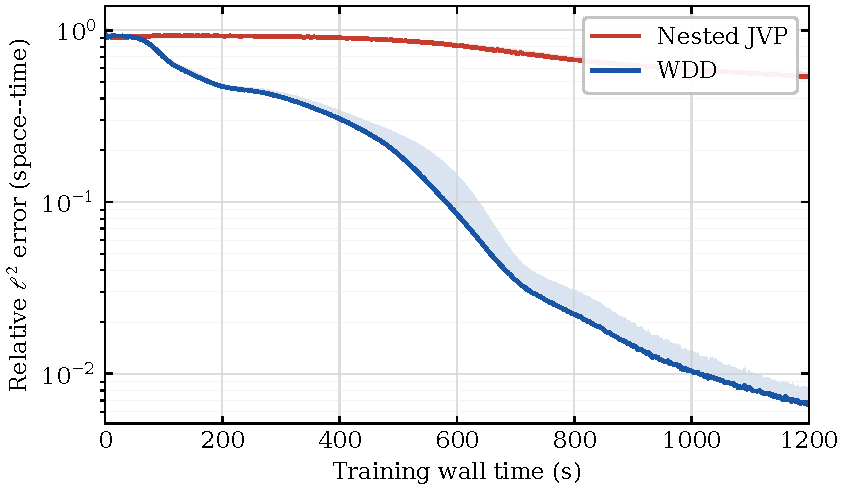
\includegraphics[width=.78\linewidth]{resampled_wall_kdv1d.pdf}
\caption{Space--time relative error during training for the one-dimensional
KdV equation \eqref{eq_num_kdv}.}
\label{fig_wall_kdv1d}
\end{figure}
\FloatBarrier

\subsubsection{Mixed-derivative PINN for a two-dimensional KdV equation}
\label{sec_num_kdv2d}

This example combines the spatial mixed derivative $u_{xxxy}$
with the space--time derivative $u_{ty}$.
We consider the KdV-type equation
in~\cite[Eq.~(20)]{Shi2024stde},
\begin{equation}\label{eq_num_kdv2d}
 \begin{cases}
 u_{ty}+u_{xxxy}+3(u_xu_y)_x-u_{xx}+2u_{yy}=0,
     &(x,y)\in(-1,1)^2,\quad t\in(0,1),\\
 u(x,y,0)=u_\star(x,y,0),
     &(x,y)\in[-1,1]^2,\\
 u(-1,y,t)=u_\star(-1,y,t),
     &y\in[-1,1],\quad t\in(0,1),\\
 u(1,y,t)=u_\star(1,y,t),
     &y\in[-1,1],\quad t\in(0,1),\\
 \partial_xu(1,y,t)=\partial_xu_\star(1,y,t),
     &y\in[-1,1],\quad t\in(0,1),\\
 u(x,-1,t)=u_\star(x,-1,t),
     &x\in[-1,1],\quad t\in(0,1),\\
 \partial_yu(x,-1,t)=\partial_yu_\star(x,-1,t),
     &x\in[-1,1],\quad t\in(0,1).
 \end{cases}
\end{equation}
The exact oblique-kink solution is
\begin{equation}\label{eq_num_kdv2d_exact}
 u_\star(x,y,t)=\tanh\bigl((x+y)/2-t\bigr).
\end{equation}
Only the PDE is taken from the cited work; the domain, exact solution,
and initial--boundary conditions specify the present benchmark. Define
the PDE residual by
\begin{equation*}
 r_\theta(x,y,t):=(u_\theta)_{ty}+(u_\theta)_{xxxy}
 +3\partial_x\bigl[(u_\theta)_x(u_\theta)_y\bigr]
 -(u_\theta)_{xx}+2(u_\theta)_{yy},
\end{equation*}
and the initial and boundary penalty by
\begin{align*}
 \mathcal J_b(\theta)
   ={}&\operatorname{MSE}_{x,y}
        \bigl[u_\theta(x,y,0)-u_\star(x,y,0)\bigr]\\
     &+\operatorname{MSE}_{y,t}
        \bigl[u_\theta(-1,y,t)-u_\star(-1,y,t)\bigr]\\
     &+\operatorname{MSE}_{y,t}
        \bigl[u_\theta(1,y,t)-u_\star(1,y,t)\bigr]\\
     &+\operatorname{MSE}_{x,t}
        \bigl[u_\theta(x,-1,t)-u_\star(x,-1,t)\bigr]\\
     &+\operatorname{MSE}_{y,t}
        \bigl[\partial_xu_\theta(1,y,t)-\partial_xu_\star(1,y,t)\bigr]\\
     &+\operatorname{MSE}_{x,t}
        \bigl[\partial_yu_\theta(x,-1,t)-\partial_yu_\star(x,-1,t)\bigr],
\end{align*}
where the subscripts of $\operatorname{MSE}$ indicate the coordinates
over which the sample mean squared errors are taken. The objective is
\begin{equation}\label{eq_num_kdv2d_loss}
 \mathcal J_{\rm 2D}(\theta)=\langle r_\theta^2\rangle_r
       +10\mathcal J_b(\theta).
\end{equation}
There is no residual-gradient penalty.

Using \eqref{eq_num_quartic_identity} with $t$ replaced by $y$,
together with
\begin{equation}\label{eq_num_kdv2d_time_identity}
 yt=\tfrac14\bigl[(y+t)^2-(y-t)^2\bigr],
\end{equation}
Proposition~\ref{prop_bridge} gives
\begin{align}\label{eq_num_kdv2d_reconstruction}
 u_{xxxy}&=4\bigl[T_4(1,1,0)-T_4(1,-1,0)\bigr]
 -\tfrac12\bigl[T_4(1,2,0)-T_4(1,-2,0)\bigr],\\
 u_{ty}&=\tfrac12\bigl[T_2(0,1,1)-T_2(0,1,-1)\bigr].\notag
\end{align}
Algorithm~\ref{alg_homogeneous} evaluates Taylor expansions along six
real directions. Their lower-order coefficients also recover
$u_x,u_y,u_{xx},u_{xy},u_{yy}$.

The results in Table~\ref{tab_wall_kdv2d} and
Figure~\ref{fig_wall_kdv2d} show that the computational advantage
of the WDD method persists for this mixed-derivative objective.

\begin{table}[htbp]
\centering
\scriptsize
\setlength{\tabcolsep}{3pt}
\caption{Numerical results for the two-dimensional KdV equation
\eqref{eq_num_kdv2d}.}
\label{tab_wall_kdv2d}
\begin{tabular}{@{}lcccc@{}}
\toprule
Method & Updates & \shortstack{Space--time\\$\operatorname{RE}$} & \shortstack{Terminal\\$\operatorname{RE}$} & $S_{\mathrm{iter}}$ \\
\midrule
Nested JVP & $2992.0 \pm 86.8$ & $4.395\times10^{-2}\pm9.677\times10^{-3}$ & $6.125\times10^{-2}\pm1.233\times10^{-2}$ & $1$ \\
WDD & $16653.6 \pm 152.2$ & $1.365\times10^{-3}\pm3.287\times10^{-4}$ & $2.313\times10^{-3}\pm6.813\times10^{-4}$ & $5.57 \pm 0.18$ \\
\bottomrule
\end{tabular}

\end{table}

\begin{figure}[htbp]
\centering
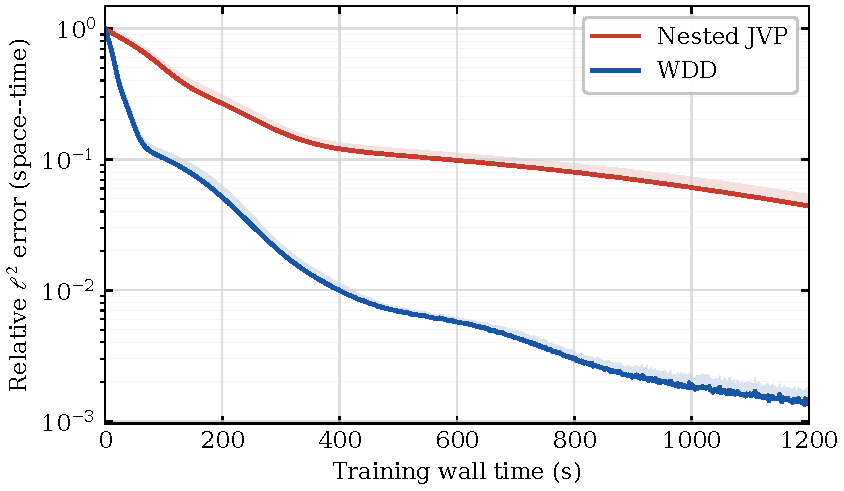
\includegraphics[width=.78\linewidth]{resampled_wall_kdv2d.pdf}
\caption{Space--time relative error during training for the two-dimensional
KdV equation \eqref{eq_num_kdv2d}.}
\label{fig_wall_kdv2d}
\end{figure}
\FloatBarrier

\subsubsection{Fourth-order Cahn--Hilliard equation}\label{sec_num_ch}

This example tests Taylor coefficient reuse for the Laplacian and
biharmonic operators in a nonlinear PDE.
We solve the Cahn--Hilliard problem
\begin{equation}\label{eq_num_ch}
 \begin{cases}
 u_t-\Delta(u^3-u)+0.01\Delta^2u=f(x,y,t),
       &(x,y)\in(0,\pi)^2,\quad t\in(0,1),\\
 u(x,y,0)=u_\star(x,y,0),
       &(x,y)\in[0,\pi]^2,\\
 \partial_{\bm n} u=0,\quad\partial_{\bm n}\Delta u=0,
       &\begin{aligned}
          (x,y)&\in\partial\bigl((0,\pi)^2\bigr),\\
          t&\in(0,1).
        \end{aligned}
 \end{cases}
\end{equation}
Here $\nabla$ and $\Delta$ act on the spatial coordinates, and $\bm n$
is the outward spatial unit normal.
The exact solution contains three spatial modes,
\begin{equation}\label{eq_num_ch_exact}
 u_\star(x,y,t)=e^{-t}\left[
 \tfrac12\cos x\cos y+
 \tfrac14\cos(2x)\cos y+
 \tfrac14\cos x\cos(2y)\right].
\end{equation}
The source $f$ is obtained by substituting \eqref{eq_num_ch_exact} into
the PDE in \eqref{eq_num_ch}.

Expanding the nonlinear Laplacian gives the residual
\begin{equation}\label{eq_num_ch_residual}
 r_\theta(x,y,t):=(u_\theta)_t-(3u_\theta^2-1)\Delta u_\theta
          -6u_\theta|\nabla u_\theta|^2
          +0.01\Delta^2u_\theta-f.
\end{equation}
Let $\mathcal F$ denote the four spatial boundary faces. The initial
and boundary penalty is
\begin{align*}
 \mathcal J_b(\theta)
   ={}&\operatorname{MSE}_{x,y}
        \bigl[u_\theta(x,y,0)-u_\star(x,y,0)\bigr]\\
     &+\frac14\sum_{F\in\mathcal F}
       \left\{\operatorname{MSE}_{F,t}\bigl[\partial_{\bm n}u_\theta\bigr]
       +\operatorname{MSE}_{F,t}
          \bigl[\partial_{\bm n}\Delta u_\theta\bigr]\right\},
\end{align*}
where $\operatorname{MSE}_{F,t}$ is evaluated over sampled points on
$F\times(0,1)$. The objective is
\begin{equation}\label{eq_num_ch_loss}
 \mathcal J_{\rm CH}(\theta)=\langle r_\theta^2\rangle_r
 +10\mathcal J_b(\theta).
\end{equation}
There is no additional mass, energy, or residual-gradient penalty.

For the spatial operators, we use the identities
\begin{align}\label{eq_num_ch_symbols}
 (x^2+y^2)^2&=\dfrac{8}{9}\left[x^4+\left(\frac{x+\sqrt3y}{2}\right)^4
                       +\left(\frac{-x+\sqrt3y}{2}\right)^4\right],\\
 x^2+y^2&=\dfrac{2}{3}\left[x^2+\left(\frac{x+\sqrt3y}{2}\right)^2
                       +\left(\frac{-x+\sqrt3y}{2}\right)^2\right].\notag
\end{align}
Writing $\bv_r$ for the coefficient vectors of these three linear forms
in $(x,y,t)$, Proposition~\ref{prop_bridge} gives
\begin{equation}\label{eq_num_ch_reconstruction}
 \Delta^2u_\theta=\tfrac{64}{3}\sum_{r=1}^3T_4(\bv_r),
 \qquad
 \Delta u_\theta=\tfrac43\sum_{r=1}^3T_2(\bv_r).
\end{equation}
The quadratic identity also yields
$|\nabla u_\theta|^2=\tfrac23\sum_{r=1}^3[T_1(\bv_r)]^2$.
Algorithm~\ref{alg_homogeneous} therefore evaluates Taylor expansions
along three real spatial directions; time and boundary derivatives
use coordinate JVPs in both methods.

Table~\ref{tab_wall_ch2d} and Figure~\ref{fig_wall_ch2d} show lower
mean final errors with the WDD method, although
$S_{\mathrm{iter}}$ is smaller than in the KdV examples.

\begin{table}[htbp]
\centering
\scriptsize
\setlength{\tabcolsep}{3pt}
\caption{Numerical results for the Cahn--Hilliard equation
\eqref{eq_num_ch}.}
\label{tab_wall_ch2d}
\begin{tabular}{@{}lcccc@{}}
\toprule
Method & Updates & \shortstack{Space--time\\$\operatorname{RE}$} & \shortstack{Terminal\\$\operatorname{RE}$} & $S_{\mathrm{iter}}$ \\
\midrule
Nested JVP & $628.4 \pm 13.8$ & $3.032\times10^{-1}\pm2.792\times10^{-2}$ & $4.956\times10^{-1}\pm7.889\times10^{-2}$ & $1$ \\
WDD & $1201.0 \pm 30.0$ & $1.601\times10^{-1}\pm3.638\times10^{-2}$ & $3.301\times10^{-1}\pm7.128\times10^{-2}$ & $1.91 \pm 0.07$ \\
\bottomrule
\end{tabular}

\end{table}

\begin{figure}[htbp]
\centering
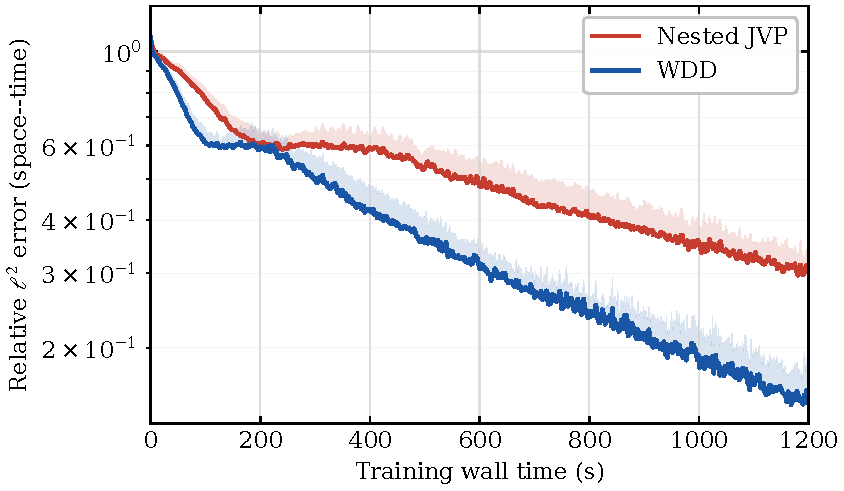
\includegraphics[width=.78\linewidth]{resampled_wall_ch2d.pdf}
\caption{Space--time relative error during training for the Cahn--Hilliard
equation \eqref{eq_num_ch}.}
\label{fig_wall_ch2d}
\end{figure}

Across the PDE experiments, the WDD method completes more
updates and attains lower mean errors under the same training-time budget,
with both interior and constraint training points resampled at every update.

\FloatBarrier

\section{Conclusion}\label{sec_concl}

Polynomial symbols yield exact directional representations of high-order
derivatives. Waring-rank theory and the roots-of-unity decomposition give
minimum-length complex formulas for mixed partials. The WDD method evaluates
these representations by batched Taylor propagation, while real power-sum
identities allow Taylor coefficients to be reused across PDE derivative terms.
The experiments show faster individual-partial evaluation and more PINN updates
under the same training-time budget. With interior and constraint points
resampled at every update, the WDD method attains lower mean errors for the
tested KdV and Cahn--Hilliard problems.

%% ====================================================================
%%  APPENDIX
%% ====================================================================
\appendix

\section{Algebraic verification and explicit schedules}\label{sec_schedules}

This appendix verifies the cited roots-of-unity decomposition in the notation
of this paper and collects several explicit schedules for representative
derivative patterns. The formulas in Appendix~\ref{sec_lowschedules} are
instances of the representation evaluated by the implementation.

\subsection{Roots-of-unity filter}\label{sec_filter}

\begin{lemma}\label{lem_filter}
    For every integer $m \ge 1$ and every integer $k$,
    \begin{equation}\label{eq_filter}
        \sum_{\zeta \in U_m}\zeta^k
        =
        \begin{cases}
            m, & m\mid k,\\
            0, & m\nmid k.
        \end{cases}
    \end{equation}
\end{lemma}

\begin{proof}
    Let $\omega := \exp(2\pi\mathrm{i}/m)$, so that every element of $U_{m}$ is
    $\omega^{\ell}$ for exactly one $\ell \in \{0, \ldots, m-1\}$ and
    \begin{equation*}
        \sum_{\zeta \in U_{m}} \zeta^{k} = \sum_{\ell=0}^{m-1}\bigl(\omega^{k}\bigr)^{\ell}.
    \end{equation*}
    If $m \mid k$, then $\omega^{k} = 1$ and the sum equals $m$. If $m \nmid k$,
    then $\omega^{k} \ne 1$, and the finite geometric series gives
    \begin{equation*}
        \sum_{\ell=0}^{m-1}\bigl(\omega^{k}\bigr)^{\ell} = \frac{1-\omega^{km}}{1-\omega^{k}} = 0,
    \end{equation*}
    since $\omega^{m} = 1$.
\end{proof}

\subsection{Verification of the explicit monomial decomposition}
\label{sec_monomial_verification}

For completeness, we verify the decomposition \eqref{eq_scaled_waring} of
Buczyńska, Buczyński, and Teitler~\cite[Sec.~2, Eq.~(8)]{BBT2013} in the
notation used here. For
$\beta=(\beta_0,\ldots,\beta_n)\in\N_0^{n+1}$ with $\abs{\beta}=p$, the
coefficient of $\bz^\beta$ on the right-hand side of
\eqref{eq_scaled_waring} is
\begin{equation}\label{eq_monomial_coefficient}
    \frac{\nu!}{\prod_{j=1}^{n}(\nu_j+1)}
    \binom{p}{\beta}
    \prod_{j=1}^{n}
    \left(
        \sum_{\zeta_j\in U_{\nu_j+1}}
        \zeta_j^{\beta_j+1}
    \right).
\end{equation}
Lemma~\ref{lem_filter} shows that the product can be nonzero only if
\begin{equation*}
    \beta_j\equiv \nu_j\pmod{\nu_j+1},
    \qquad j=1,\ldots,n.
\end{equation*}
Each $\beta_j$ is therefore either $\nu_j$ or at least $2\nu_j+1$. If
$\beta_j\geq2\nu_j+1$ for some $j\geq1$, then the remaining congruences give
$\beta_k\geq \nu_k$ and hence
\begin{equation*}
    \beta_0
    =p-\sum_{k=1}^{n}\beta_k
    \leq \nu_0-\nu_j-1
    <0,
\end{equation*}
which contradicts $\beta_0\geq0$. Thus $\beta_j=\nu_j$ for
$j=1,\ldots,n$, and $\abs{\beta}=p$ then gives $\beta_0=\nu_0$.
Consequently, the coefficient in \eqref{eq_monomial_coefficient} vanishes
unless $\beta_j=\nu_j$ for every $j=0,\ldots,n$. In that case, the
coefficient equals
\begin{equation*}
    \frac{\nu!}{\prod_{j=1}^{n}(\nu_j+1)}
    \frac{p!}{\nu!}
    \prod_{j=1}^{n}(\nu_j+1)
    =p!.
\end{equation*}
This proves \eqref{eq_scaled_waring}.

\subsection{Explicit low-order schedules}\label{sec_lowschedules}

The following formulas are low-order instances of
\eqref{eq_optimal_representation}. Let $\bm e_i$ denote the $i$th coordinate
vector in $\C^d$.

For the pure derivative $\partial_{1}^{p}$ we have $n = 0$, the schedule has one
direction, and $\Tp$ is evaluated once,
\begin{equation}\label{eq_sched_pure}
    \partial_{1}^{p}u(\bx) = p!\,\Tp(\bx; \bm e_{1}).
\end{equation}

For the mixed second derivative, $(\nu_0,\nu_1)=(1,1)$ and
\eqref{eq_optimal_representation} gives
\begin{equation}\label{eq_two_point}
    \partial_1\partial_2u(\bx)
    =
    \frac{1}{2}T_2(\bx;\bm e_1+\bm e_2)
    -
    \frac{1}{2}T_2(\bx;\bm e_1-\bm e_2).
\end{equation}
The two directions in \eqref{eq_two_point} attain the minimum in
\eqref{eq_directional_rank}.

For the fourth-order mixed derivative $\partial_{1}^{2}\partial_{2}^{2}$ we
have $n = 1$ and $(\nu_0,\nu_1)=(2,2)$; with $\omega :=
\exp(2\pi\mathrm{i}/3)$ and $U_{3} = \{1, \omega, \omega^{2}\}$, formula
\eqref{eq_optimal_representation} gives the three directions
\begin{equation}\label{eq_sched_22}
    \partial_{1}^{2}\partial_{2}^{2}u(\bx) = \frac{4}{3}\sum_{\zeta \in U_{3}} \zeta\,T_4(\bx;\, \bm e_{1}+\zeta \bm e_{2}).
\end{equation}

For the sixth-order mixed derivative $\partial_{1}^{2}\partial_{2}^{4}$ we
have $n = 1$ and $(\nu_0,\nu_1)=(2,4)$; with $U_{5}$ the fifth roots of
unity, \eqref{eq_optimal_representation} takes the coordinate of smaller
exponent as base and gives the five directions
\begin{equation}\label{eq_sched_24}
    \partial_{1}^{2}\partial_{2}^{4}u(\bx) = \frac{48}{5}\sum_{\zeta \in U_{5}} \zeta\,T_6(\bx;\, \bm e_{1}+\zeta \bm e_{2}).
\end{equation}
The companion term $\partial_{1}^{4}\partial_{2}^{2}$ is the same formula with
the two coordinates exchanged. The polynomial identity corresponding to
\eqref{eq_sched_24} reads
\begin{equation}\label{eq_sched_24_poly}
    6!\,z_{0}^{2}z_{1}^{4} = \frac{48}{5}\sum_{\zeta \in U_{5}} \zeta\,(z_{0}+\zeta z_{1})^{6},
\end{equation}
and it can be checked directly: the coefficient of
$z_{0}^{\beta_{0}}z_{1}^{\beta_{1}}$ on the right-hand side contains the factor
$\sum_{\zeta \in U_{5}}\zeta^{1+\beta_{1}}$, which by Lemma~\ref{lem_filter} is
nonzero only when $\beta_{1} \equiv 4 \pmod{5}$.
Together with $\beta_{0}+\beta_{1} = 6$ this forces $\beta = (2,4)$, and the
surviving constant is $\tfrac{48}{5} \cdot \tfrac{6!}{2!\,4!} \cdot 5 = 720 =
6!$. The three-variable pattern $(2,2,2)$ of Table~\ref{tab_patterns} is the
same construction with two cube-root factors and nine directions.

Table~\ref{tab_patterns} lists the minimum number of directions for
representative exponent patterns.

\begin{table}[htbp]
\centering
\footnotesize
\caption{Minimum numbers of directions for representative monomial derivatives.}
\label{tab_patterns}
\begin{tabular}{@{}llr@{}}
\toprule
pattern & example derivative & $R_{\C}$ \\
\midrule
$(p)$        & $\partial_{1}^{p}u$ & $1$ \\
$(2,1)$      & $u_{112}$    & $3$ \\
$(1,1,1)$    & $u_{123}$    & $4$ \\
$(3,1)$      & $u_{1112}$   & $4$ \\
$(2,2)$      & $u_{1122}$   & $3$ \\
$(2,1,1)$    & $u_{1123}$   & $6$ \\
$(1,1,1,1)$  & $u_{1234}$   & $8$ \\
$(4,2)$      & $u_{111122}$ & $5$ \\
$(2,2,2)$    & $u_{112233}$ & $9$ \\
$(1^{6})$    & $u_{123456}$ & $32$ \\
\bottomrule
\end{tabular}
\end{table}

%% ====================================================================
%%  REFERENCES
%% ====================================================================
\FloatBarrier
\bibliographystyle{siamfull}
\bibliography{jsc_paper_main}

\end{document}
